\section{Auswertung}
Abbildung \ref{fig:spektrum} zeigt das Absortpionsspektrumpektrum des ${}^{137}\text{Cs}$-Strahlers.
Zur Erstellung der Abbildungen wird das \texttt{python}-Paket \texttt{matplotlib} \cite{Hunter:2007} verwendet, die Auswertung erfolgt
mit dem Paket \texttt{numpy} \cite{harris2020array}. Die Fehlerrechnung zur Berücksichtigung der Messunsicherheiten wird mit dem Paket \texttt{uncertainties} \cite{uncertainties}
automatisiert.
Über 
\begin{equation*}
    N = \frac{C}{t}
\end{equation*}
wird über die Anzahl der Counts $C$ auf die Zählrate $N$ umgerechnet, die als Maß für die Intensität
verwendet werden kann.
Deutlich erkennbar ist der Photopeak bei Kanalnummer 128, entsprechend der Energie $E= 661,7 \text{ keV}$ 
und die Compton-Kante im Bereich der Kanalnummern 85 bis 105. 
\begin{figure}
    \centering
    \includegraphics[width = \linewidth]{Leermessung.pdf}
    \caption{Spektrum der ${}^{137}\text{Cs}$-Quelle. Aufgetragen sind die Zählraten der einzelnen
    Kanäle mit den entsprechenden Kanalnummern. Die grüne Linie markiert den Photopeak bei  
    Kanalnummer 128 und der charakteristischen Energie $E_\gamma = 661,7 \text{ keV}$. Die Compton-
    Kante liegt im Bereich der Kanalnummern 85 bis 105. Erstellt mit dem \texttt{python}-Paket \texttt{matplotlib} \cite{Hunter:2007}.}
    \label{fig:spektrum}
\end{figure}
%TO-DO:Matrix vorher einfügen, Projektionen erklären
Zur experimentellen Bestimmung der Absorptionskoeffizienten $\mu$ werden vorab die Literaturwerte bestimmt. Diese können über
\begin{equation*}
    \mu = \rho \cdot \sigma
\end{equation*}
mit dem Massenschwächungskoeffizient $\sigma$ und der Dichte $\rho$ berechnet werden. Die Massenschwächungskoeffizienten werden der NIST
Datenbank XCOM \cite{xcom} entnommen, wobei als Eingabeenergie die Energie des Photopeaks $E_\gamma = 661,7 \text{ keV}$ verwendet wird.
Die Dichten finden sich unter \cite{rsc}, \cite{delrin} und \cite{chemie}. 
Die Ergebnisse der Berechung sind in Tabelle \ref{tab:literatur} aufgeführt.
\FloatBarrier
\begin{table}[h]
    \centering
    \caption{Über den Massenschwächungskoeffizienten $\sigma$ und die Dichte $\rho$ berechnete Literaturwerte der 
    Absorptionskoeffizienten verschiedener Materialien. Die Werte für $\sigma$ sind Ref. \cite{xcom} entnommen, die Werte für 
    $\rho$ Ref. \cite{rsc}, \cite{delrin} und \cite{chemie}.}
    \label{tab:literatur}
    \begin{tabular}{l l S[table-format=1.4] S[table-format=2.2] S[table-format=1.3]}
        \toprule
        {Material} & {} & {$\sfrac{\sigma}{\si{\centi\meter\squared\per\gram}}$} & {$\sfrac{\rho}{\si{\gram\per\cubic\centi\meter}}$} & {$\sfrac{\mu}{\ \si{\per\centi\meter}}$}\\
        \midrule
        {Aluminium} & {Al}                    & 0.0747 & 2.7  & 0.202 \\
        {Blei}      & {Pb}                    & 0.1102 & 11.3 & 1.245 \\
        {Eisen}     & {Fe}                    & 0.0735 & 7.87 & 0.578 \\
        {Messing}   & {CuZn}                  & 0.0729 & 8.5  & 0.620 \\
        {Delrin}    & {$\text{CH}_2\text{O}$} & 0.0823 & 1.43 & 0.118 \\
        \bottomrule
    \end{tabular}
\end{table}
\FloatBarrier
\noindent
Die Absorptionskoeffizienten werden für die Würfel mit den Nummern 1, 3 und 4 bestimmt. Würfel 1 ist leer und besteht nur aus dem Aluminiumgehäuse.
Würfel 3 besteht nur aus einem unbekannten Material, Würfel 4 aus zwei unbekannten Materialien. 
Die gemessenen Counts $C$, Messdauer $t$, Zählraten $N$ sowie die entsprechenden Projektionen der Würfel 3 und 4 
befinden sich in den Tabellen \ref{tab:W3} und \ref{tab:W4}. In Tabelle \ref{tab:W3} sind zudem die berechneten Absorptionskoeffizienten
aufgeführt. Die Zählraten $N$ werden mit dem statistischen Fehler $\sqrt{N}$
belegt, die Messdauer wird als fehlerfrei angenommen.
Bei der Untersuchung von Würfel 1 werden bei einer Messdauer von $241.62 \text{ s}$ 
\begin{equation*}
    C = 37660
\end{equation*}
Counts gemessen.  
Die Berechnung der Absorptionskoeffizienten $\mu_i$ erfolgt über Gleichung \ref{eq:mu}. Über die Kovarianzmatrix $V[\vec{\mu}]$ ergeben sich die entsprechenden 
Unsicherheiten $\sigma_I$ als Wurzeln der Diagonalelemente
\begin{equation*}
    \sigma_{\mu_i} = \sqrt{V[\vec{\mu}_{ii}]} 
\end{equation*}
\FloatBarrier
\begin{table}[h]
    \centering
    \caption{Gemessene Counts $C$, und Messdauern $t$ sowie die entsprechenden Projektionen für Würfel 3. Aufgeführt sind außerdem die 
    daraus berechneten Zählraten als Maß für die Intensität sowie die experimentell bestimmten Werte des Absorptionskoeffizienten.}
    \label{tab:W3}
    \begin{tabular}{c S[table-format=4.0] S[table-format=3.2] S[table-format=1.2]@{${}\pm{}$} S[table-format=1.2] S[table-format=1.3]@{${}\pm{}$} S[table-format=1.3]}
        \toprule
        {Projektion} & {$C$} & {$t/\si{\s}$} & \multicolumn{2}{c}{$N/\si{\s}^{-1}$} & \multicolumn{2}{c}{$\mu /\si{\cm}^{-1}$} \\
        \midrule
        $I_2$ & 1301 & 241.24 & 5.39 & 2.32 & 1.055 & 0.311\\
        $I_7$ & 1164 & 241.24 & 4.83 & 2.20 & 1.236 & 0.219\\
        $I_8$ & 594  & 241.24 & 2.46 & 1.57 & 0.858 & 0.250\\
        \bottomrule
    \end{tabular}
\end{table}
\FloatBarrier
\noindent
Der Mittelwert der Absorptionskoeffizienten in Tabelle \ref{tab:W3} berechnet sich zu
\begin{equation}
    \label{eq:blei}
    \bar{\mu}_{W_3} = (1,05 \pm 0,15) \,\frac{1}{\text{cm}} 
\end{equation}
und lässt sich nach Vergleich mit den Literaturwerten in Tabelle \ref{tab:literatur} dem Material 
Blei zuordnen.
\FloatBarrier
\begin{table}[h]
    \centering
    \caption{Gemessene Counts $C$, und Messdauern $t$ sowie die entsprechenden Projektionen für Würfel 4, der aus neun Elementarwürfeln
    besteht. Aufgeführt sind außerdem die daraus berechneten Zählraten als Maß für die Intensität.}
    %\sisetup{table-format=1.2}
    \label{tab:W4}
    \begin{tabular}{c S[table-format=5.0] S[table-format=3.2] S[table-format=3.2]@{${}\pm{}$} S[table-format=2.2]}
        \toprule
        {Projektion} & {$C$} & {$t/\si{\s}$} & \multicolumn{2}{c}{$N/\si{\s}^{-1}$} \\
        \midrule
        $I_1$    & 30557 & 241.80 & 126.37 & 11.24 \\
        $I_2$    & 1612  & 241.42 & 6.68   & 2.58  \\
        $I_3$    & 30303 & 241.78 & 125.33 & 11.20 \\
        $I_4$    & 10235 & 241.46 & 42.39  & 6.51  \\
        $I_5$    & 9544  & 241.46 & 39.53  & 6.29  \\
        $I_6$    & 10361 & 241.48 & 42.91  & 6.55  \\
        $I_7$    & 6993  & 241.48 & 28.96  & 5.38  \\
        $I_8$    & 6196  & 241.46 & 25.66  & 5.07  \\
        $I_9$    & 9419  & 241.56 & 38.99  & 6.24  \\
        $I_{10}$ & 7478  & 241.50 & 30.96  & 5.56  \\
        $I_{11}$ & 6377  & 241.50 & 26.41  & 5.14  \\
        $I_{12}$ & 9861  & 241.54 & 40.83  & 6.39  \\
        \bottomrule
    \end{tabular}
\end{table}
\FloatBarrier
\noindent
In Tabelle \ref{tab:W4_Abk} sind die experimentell bestimmten Absorptionskoeffizienten der neun Elementarwürfel von Würfel 4 aufgeführt, dessen
Material unbekannt ist. Um aus den Absorptionskoeffizienten auf das Material rückschließen zu können, sind außerdem
die Abweichungen der experimentell bestimmten Koeffizienten von den Literaturwerten verschiedener Materialien, aufgeführt in 
Tabelle \ref{tab:literatur}, sowie zum experimentell bestimmten Absorptionskoeffizienten von Blei, angegeben. 
\FloatBarrier
\begin{table}[h]
    \centering
    \caption{Experimentell bestimmte Absorptionskoeffizienten der neun Elementarwürfel, aus denen Würfel 4 zusammengesetzt ist. Aufgeführt 
    sind außerdem die Beträge der Abweichungen zu den errechneten Literaturwerten der Materialien Aluminium, Blei, Eisen, Messing und Delrin.
    Für jeden Wert $\mu_i$ ist die betragsmäßig kleinste Abweichung, auf deren Grundlage die Zuordnung zu einem Material erfolgt, durch 
    Fettdruck hervorgehoben.}
    \label{tab:W4_Abk}
    \begin{tabular}{c S[table-format=1.3]@{${}\pm{}$} S[table-format=1.3] c c c c c c}
        \toprule
        {} & \multicolumn{2}{c}{$\mu_i /\si{\cm}^{-1}$} & {$|\Delta {\mu_\text{Fe, Lit}}|$} & {$|\Delta {\mu_\text{Al, Lit}}|$} & {$|\Delta {\mu_\text{Pb, Lit}}|$} & {$|\Delta {\mu_\text{Pb, Exp}}|$} & {$|\Delta {\mu_\text{CuZn, Lit}}|$} & {$|\Delta {\mu_{\text{CH}_2\text{O}, \text{Lit}}}|$} \\
        \midrule
        $\mu_1$ & 0.042  & 0.108 & 0.536 & 0.160 & 1.203 & 1.008 & 0.578 & \textbf{0.076} \\
        $\mu_2$ & 0.161  & 0.090 & 0.417 & \textbf{0.041} & 1.084 & 0.889 & 0.459 & 0.043 \\
        $\mu_3$ & 0.024  & 0.109 & 0.554 & 0.178 & 1.221 & 1.026 & 0.596 & \textbf{0.094} \\
        $\mu_4$ & 1.030  & 0.095 & 0.452 & 0.828 & 0.215 & \textbf{0.020} & 0.410 & 0.912 \\
        $\mu_5$ & 1.132  & 0.101 & 0.554 & 0.930 & 0.113 & \textbf{0.082} & 0.512 & 1.014 \\
        $\mu_6$ & 1.033  & 0.096 & 0.455 & 0.831 & 0.212 & \textbf{0.017} & 0.413 & 0.915 \\
        $\mu_7$ & 0.139  & 0.108 & 0.439 & 0.063 & 1.106 & 0.911 & 0.481 & \textbf{0.021} \\
        $\mu_8$ & -0.047 & 0.087 & 0.625 & 0.249 & 1.292 & 1.097 & 0.667 & \textbf{0.165} \\
        $\mu_9$ & 0.143  & 0.108 & 0.435 & 0.059 & 1.102 & 0.907 & 0.477 & \textbf{0.025} \\
        \bottomrule
    \end{tabular}
\end{table}
\FloatBarrier
\noindent
Die Zuordnung zu einem 
Material erfolgt anhand der betragskleinsten Abweichung des experimentell bestimmten Wertes (in der Tabelle hervorgehoben) zu den 
Vergleichswerten. Die so bestimmte 
Zusammensetzung von Würfel 4 ist in Abbildung \ref{fig:tikz2} dargestellt. Auf Grundlage der Werte in Tabelle \ref{tab:W4_Abk} 
lässt sich schlussfolgern, dass es sich bei dem Material der Elementarwürfel 1 bis 3 sowie 7 bis 9 um Delrin handelt, und bei dem 
Material der Elementarwürfel 4 bis 6 um Blei. 
Zu Beachten ist, dass für $\mu_2$ die Abweichung zum Absorptionskoeffizienten
von Aluminium mit $|\Delta {\mu_\text{Al, Lit}}| = 0,041$ eigentlich betragsmäßig am kleinsten ist. Da aber bekannt ist, dass der Würfel nur aus zwei verschiedenen Materialien besteht
und die Abweichung zum Absorptionskoeffizienten von Delrin mit $|\Delta {\mu_{\text{CH}_2\text{O}, \text{Lit}}}| = 0,043$ ähnlich klein ist, wird
angenommen, dass es sich auch bei dem Material von Elementarwürfel 2 um Delrin handelt. 
\begin{figure}
    \centering
    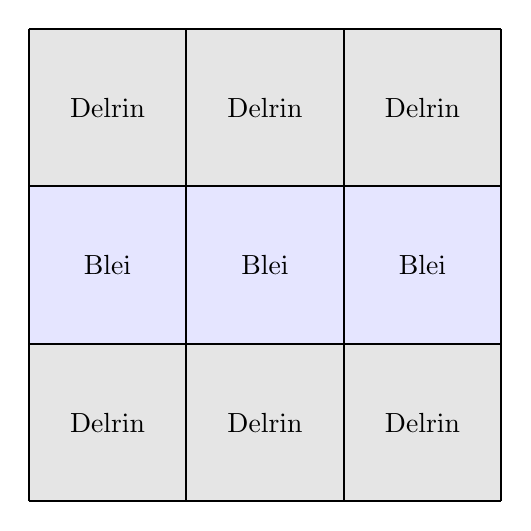
\begin{tikzpicture}
        \node[fill=gray!20, minimum size=2cm] at (1,1) {};
        \node at (1,1) {Delrin};
        \node[fill=blue!10, minimum size=2cm] at (1,3) {};
        \node at (1,3) {Blei};
        \node[fill=gray!20, minimum size=2cm] at (1,5) {};
        \node at (1,5) {Delrin};
        \node[fill=gray!20, minimum size=2cm] at (3,1) {};
        \node at (3,1) {Delrin};
        \node[fill=blue!10, minimum size=2cm] at (3,3) {};
        \node at (3,3) {Blei};
        \node[fill=gray!20, minimum size=2cm] at (3,5) {};
        \node at (3,5) {Delrin};
        \node[fill=gray!20, minimum size=2cm] at (5,1) {};
        \node at (5,1) {Delrin};
        \node[fill=blue!10, minimum size=2cm] at (5,3) {};
        \node at (5,3) {Blei};
        \node[fill=gray!20, minimum size=2cm] at (5,5) {};
        \node at (5,5) {Delrin};
        \draw[step = 2cm, thick] (0,0) grid +(6,6);
    \end{tikzpicture}
    \caption{Graphische Darstellung der untersuchten mittleren Ebene von Würfel mit den neun Elementarwürfeln sowie die Zuordnung 
    der Materialien auf Basis der experimentellen Bestimmung der Absorptionskoeffizienten. 
    Erstellt mit der \LaTeX-Erweiterung TikZ \cite{tantau:2013a.}.}
    \label{fig:tikz2}
\end{figure}

\begin{figure}
    \centering
    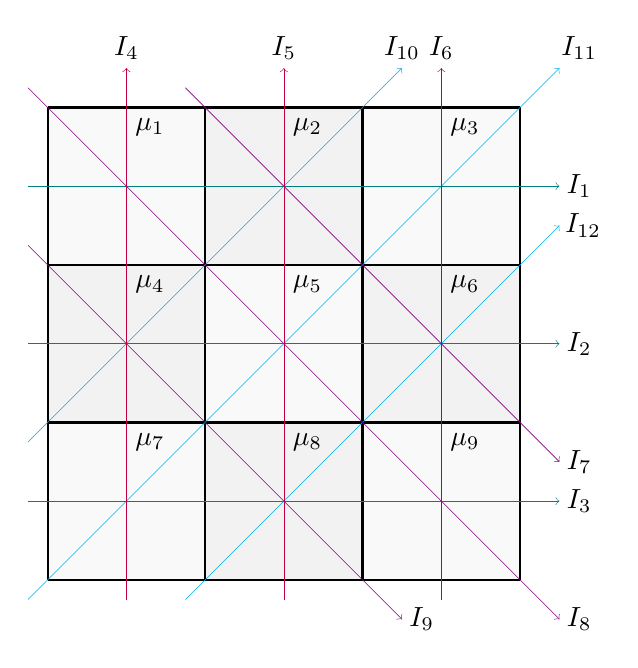
\begin{tikzpicture}

        \node[fill=gray!5, minimum size=2cm] at (1,1) {};
        \node[fill=gray!5, minimum size=2cm] at (1,5) {};
        \node[fill=gray!5, minimum size=2cm] at (5,1) {};
        \node[fill=gray!5, minimum size=2cm] at (5,5) {};
        \node[fill=gray!5, minimum size=2cm] at (3,3) {};

        \node[fill=gray!10, minimum size=2cm] at (3,1) {};
        \node[fill=gray!10, minimum size=2cm] at (1,3) {};
        \node[fill=gray!10, minimum size=2cm] at (5,3) {};
        \node[fill=gray!10, minimum size=2cm] at (3,5) {};
        \draw[step = 2cm, thick] (0,0) grid +(6,6);
        \draw[->][cyan, very thin] (-0.25,-0.25)--(6.5,6.5);
        \node at (6.75,6.75) {$I_{11}$};
        \draw[->][cyan, very thin] (-0.25,1.75)--(4.5,6.5);
        \node at (4.5,6.75) {$I_{10}$};
        \draw[->][cyan, very thin] (1.75,-0.25)--(6.5,4.5);
        \node at (6.8,4.5) {$I_{12}$};
        \draw[->][violet, very thin] (1.75,6.25)--(6.5,1.5);
        \node at (6.75,1.5) {$I_{7}$};
        \draw[->][violet, very thin] (-0.25,6.25)--(6.5,-0.5);
        \node at (6.75,-0.5) {$I_{8}$};
        \draw[->][violet, very thin] (-0.25,4.25)--(4.5,-0.5);
        \node at (4.75,-0.5) {$I_{9}$};
        \draw[->][teal, very thin] (-0.25,5)--(6.5,5);
        \node at (6.75,5) {$I_{1}$};
        \draw[->][teal, very thin] (-0.25,3)--(6.5,3);
        \node at (6.75,3) {$I_{2}$};
        \draw[->][teal, very thin] (-0.25,1)--(6.5,1);
        \node at (6.75,1) {$I_{3}$};
        \draw[->][purple, very thin] (1,-0.25)--(1,6.5);
        \node at (1,6.75) {$I_{4}$};
        \draw[->][purple, very thin] (3,-0.25)--(3,6.5);
        \node at (3,6.75) {$I_{5}$};
        \draw[->][purple, very thin] (5,-0.25)--(5,6.5);
        \node at (5,6.75) {$I_{6}$};
        \node at (1.3,1.75) {$\symbf{\mu_7}$};
        \node at (1.3,3.75) {$\symbf{\mu_4}$};
        \node at (1.3,5.75) {$\symbf{\mu_1}$};
        \node at (3.3,1.75) {$\symbf{\mu_8}$};
        \node at (3.3,3.75) {$\symbf{\mu_5}$};
        \node at (3.3,5.75) {$\symbf{\mu_2}$};
        \node at (5.3,1.75) {$\symbf{\mu_9}$};
        \node at (5.3,3.75) {$\symbf{\mu_6}$};
        \node at (5.3,5.75) {$\symbf{\mu_3}$};
    \end{tikzpicture}
    \caption{}
    \label{fig:tikz1}
\end{figure}